\documentclass[aspectratio=169]{beamer}

\usepackage[utf8]{inputenc}
\usepackage[T1]{fontenc}
\usepackage[brazil]{babel}
\usepackage{amsmath, amssymb}
\usepackage{graphicx}
\usepackage{booktabs}
\usepackage{siunitx}
\usepackage{hyperref}

\usetheme{Berlin}
\definecolor{myprimary}{RGB}{0,90,150} % exemplo: azul escuro customizado
\setbeamercolor{structure}{fg=myprimary} % define a cor primária dos elementos principais
\setbeamertemplate{navigation symbols}{}

\title{Índices de Representação Descritiva (IRD), Profissionalismo Político (IPP) e Falar Sincero (IFS)}
\author{Acácio Vasconcelos Telechi}
\date{\today}

\begin{document}

\begin{frame}
  \titlepage
\end{frame}

\begin{frame}{Agenda}
  \tableofcontents
\end{frame}

\section{Visão Geral}
  \begin{frame}{Motivação e visão geral}
    \begin{itemize}
      \item IRD: mede quão próxima está a composição observada do alvo populacional (e.g., paridade de gênero).
      \item IPP: sintetiza comprometimento institucional e carreira/capital político.
      \item \textit{IFS: mede a proximidade das postagens de um parlamentar com conteúdos comprovadamente falsos por agências de checagem de notícias}.
      \item Uso: monitoramento temporal, comparação entre legislaturas e caracterização de subgrupos.
    \end{itemize}
  \end{frame}

% ----------------------------------------------------------------------------
\section{IRD}

  \begin{frame}{Conceito e dimensões}
    \begin{itemize}
      \item IRD: mede quão próxima está a composição observada do alvo populacional (e.g., paridade de gênero).
      \item Categorias $c$ com proporções-alvo $\{p_c\}$ (e.g., \texttt{F/M}).
      \item Pesos individuais refletem contribuição para aproximar a amostra do alvo.
      \item Síntese pelo desvio médio em relação a $w_i=1$ (neutralidade).
    \end{itemize}
  \end{frame}

  \begin{frame}{Construção: pesos e índice}
    Considere $X\in\{0,1\}^{N\times C}$, $n_c=\sum_i X_{ic}$.
    \begin{align*}
      \tilde{w}_i &= \sum_{c=1}^{C} X_{ic}\,\frac{p_c}{n_c}, &
      w_i &= \tilde{w}_i\cdot \frac{N}{\sum_{j=1}^{N}\tilde{w}_j} \\
      I_{\text{ajuste}} &= 1 - \frac{1}{N}\sum_{i=1}^{N}\big|w_i - 1\big|\,.
    \end{align*}
    \begin{itemize}
      \item $\sum_i w_i=N$. Se a amostra coincide com o alvo, $w_i=1$ e $I_{\text{ajuste}}=1$.
    \end{itemize}
  \end{frame}

  \begin{frame}{Calculadora IRD}
    \texttt{EqualityIndexCalculator} fornece:
    \begin{itemize}
      \item Normalização do índice: Gini (default), limites teóricos, empíricos, entropia.
      \item Normalização dos pesos: z-score (default), min--max, robusta, rank.
      \item Pipeline completo via \texttt{calculate(\,)}.
    \end{itemize}
  \end{frame}

  \begin{frame}{Aplicação}
    \begin{itemize}
      \item Exemplo de gênero com alvo populacional $p_F=0{,}52$, $p_M=0{,}48$ (proporções reais).
      \item Saídas: pesos individuais e $I_{\text{ajuste}}$ calculados por legislatura.
      \item Generaliza para múltiplas categorias (e.g., cor/raça); ignora $n_c=0$ para evitar divisão por zero.
    \end{itemize}
  \end{frame}

  \begin{frame}{Aplicação}
    \begin{center}
      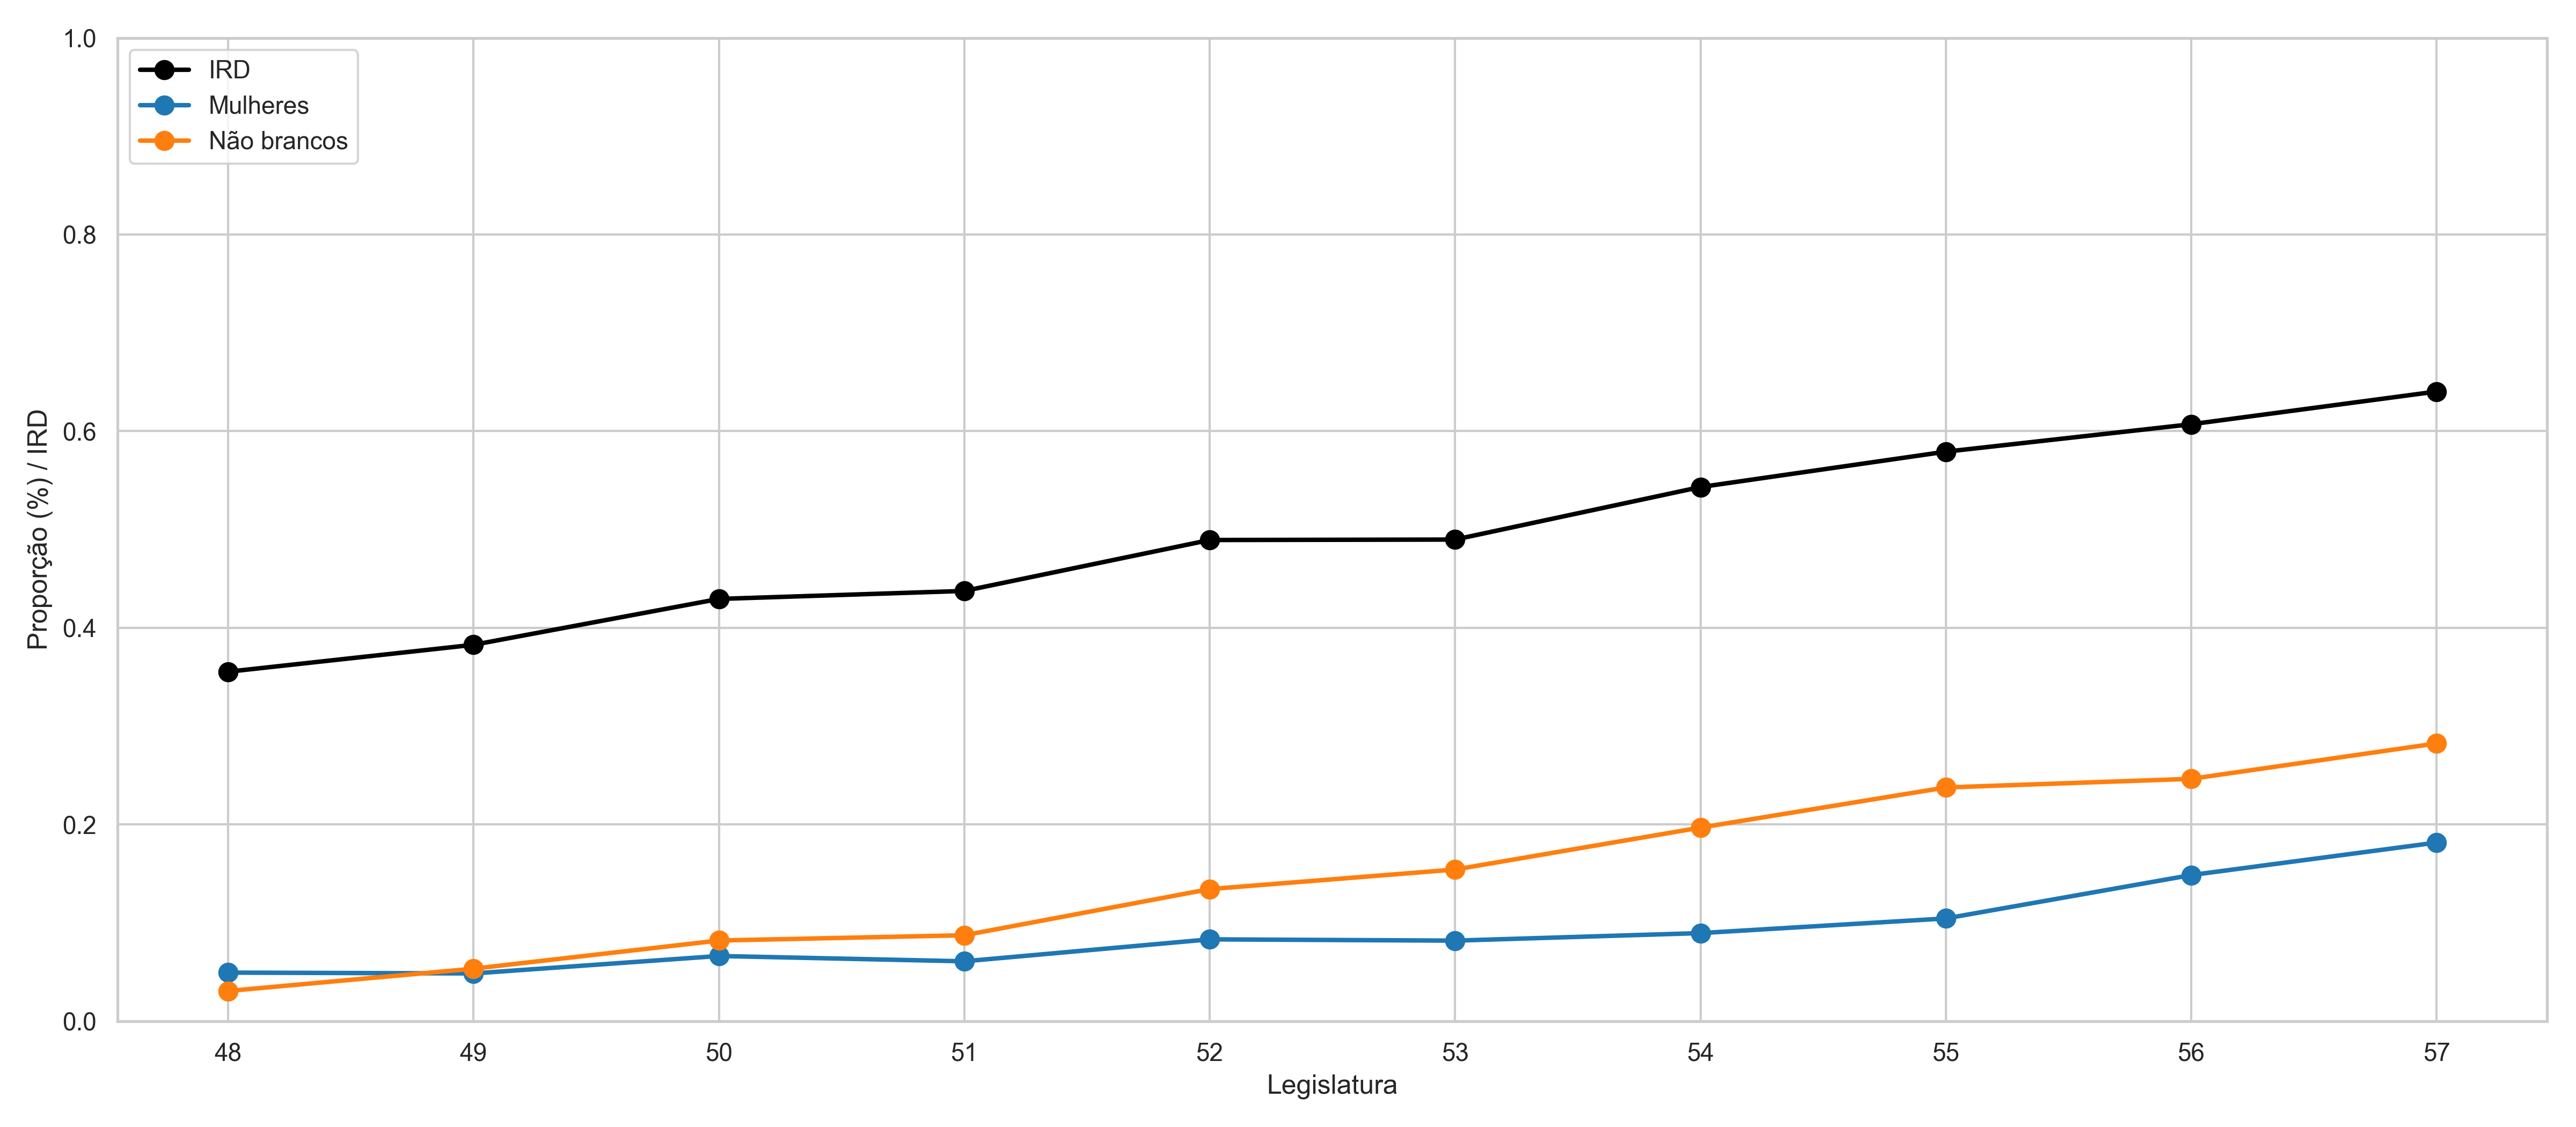
\includegraphics[width=0.90\linewidth]{figures/equality_index.png}
    \end{center}
  \end{frame}

  \begin{frame}{Aplicação}
    \begin{center}
      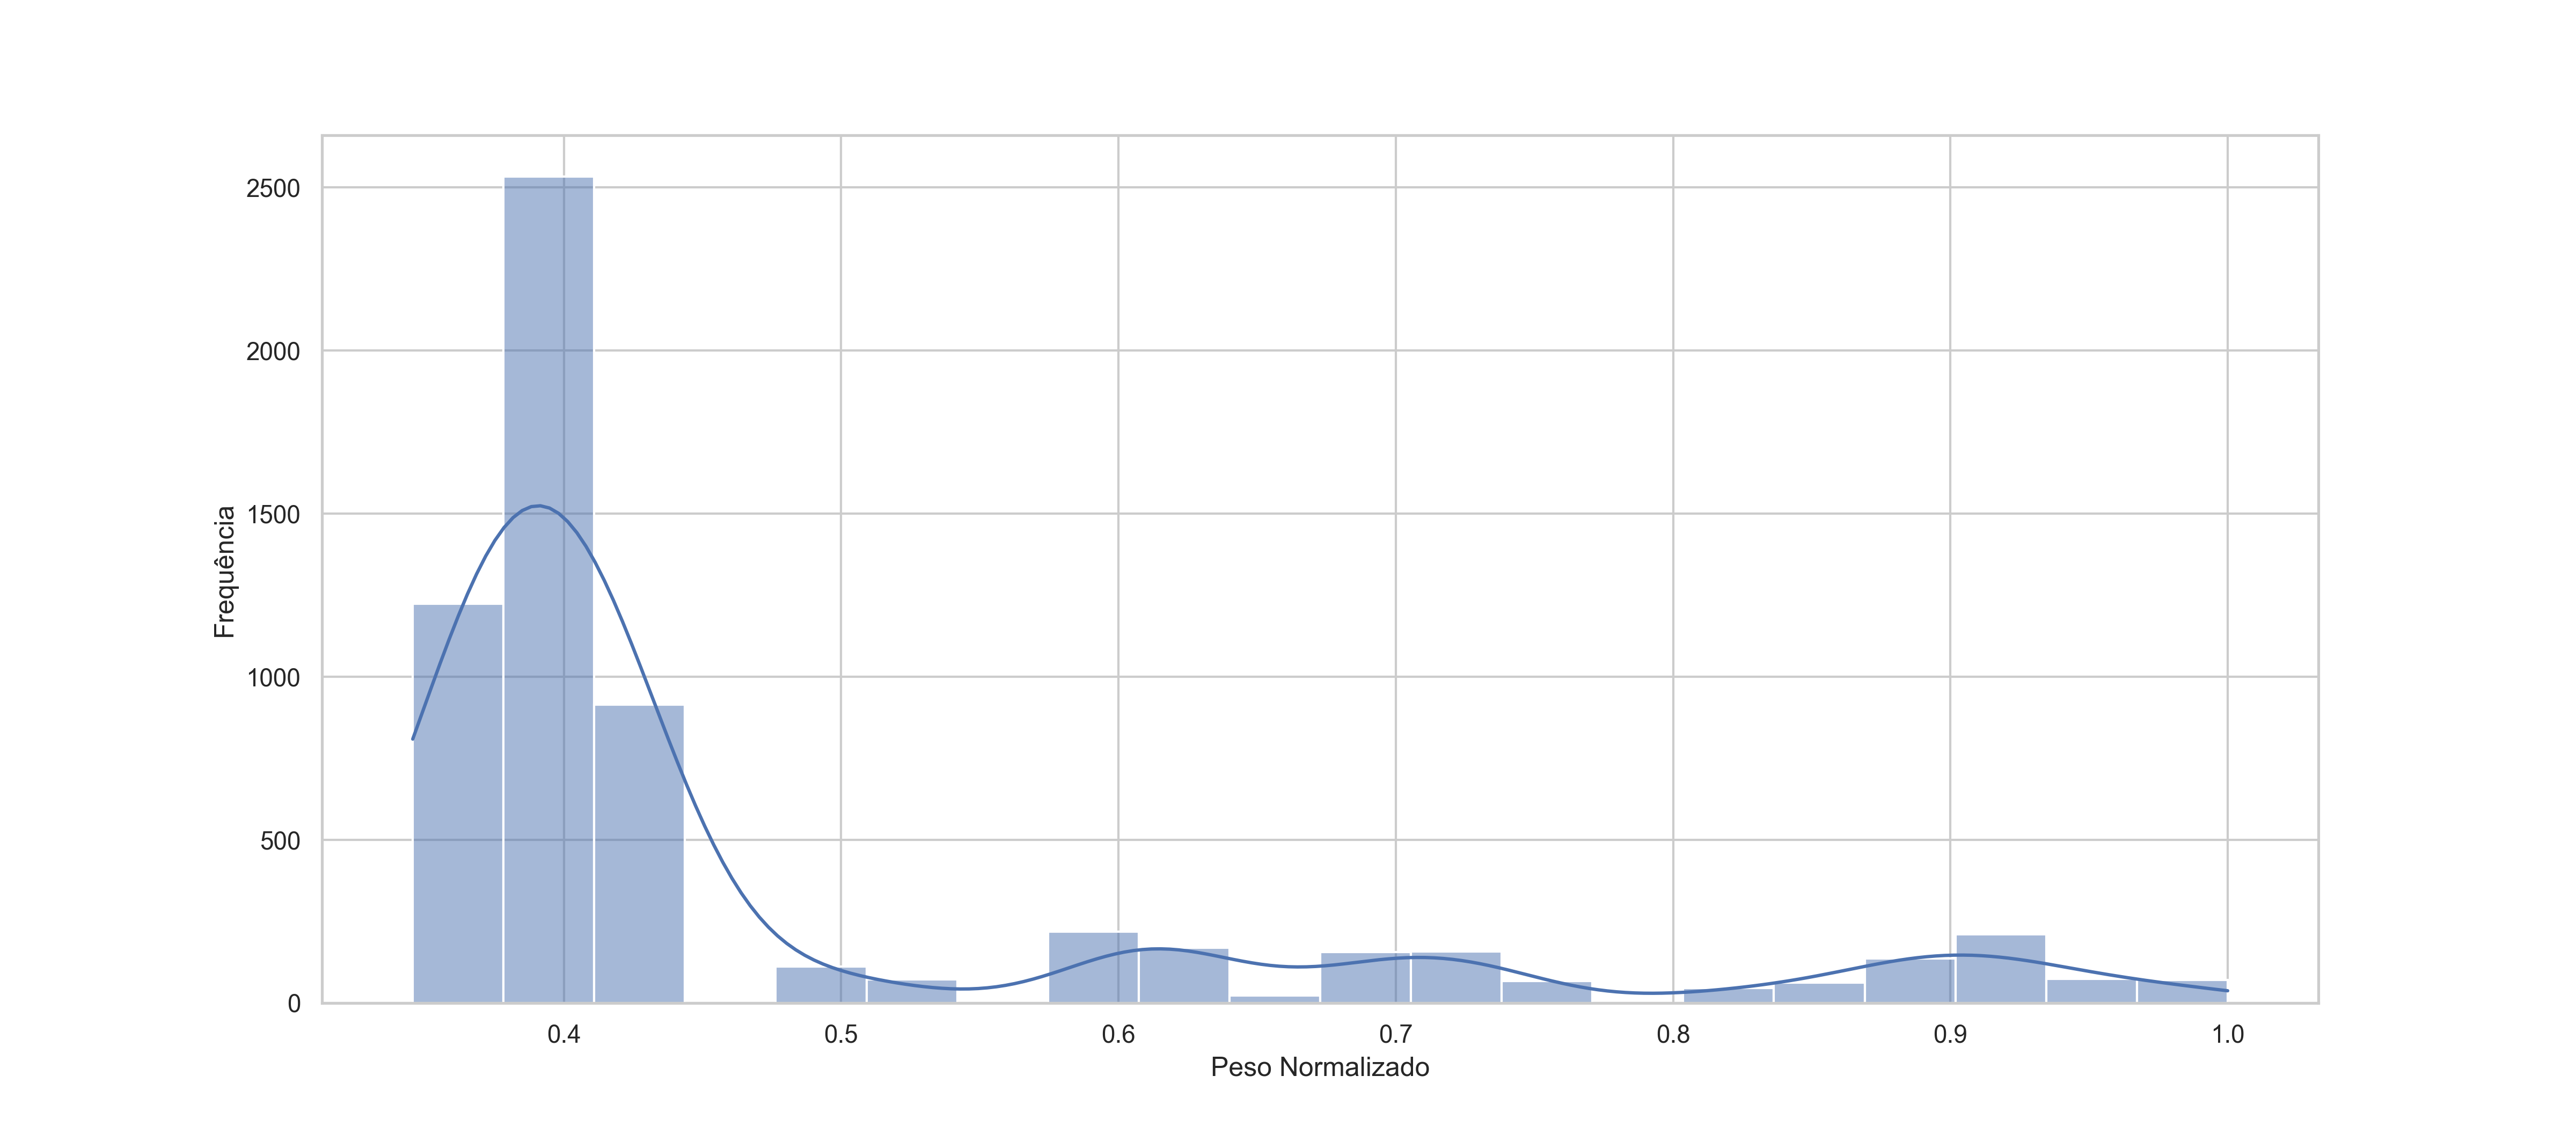
\includegraphics[width=0.90\linewidth]{figures/equality_weights_normalized.png}
    \end{center}
  \end{frame}

% ----------------------------------------------------------------------------
\section{IPP}

  \begin{frame}{Conceito e dimensões}
    \begin{itemize}
      \item \textbf{Especialização Legislativa}: lideranças, presidências, relatorias.
      \item \textbf{Carreira Parlamentar}: tempo de atuação, mandatos subnacionais, fidelidade em eleições gerais.
    \end{itemize}
  \end{frame}

  \begin{frame}{Variáveis e normalização}
    \begin{itemize}
      \item Variáveis binárias: mesa, colégio de líderes, presença em comissões, fidelidade.
      \item Variáveis contínuas: tempo de atuação, relatorias - transformadas $\ln(\text{X}+1)$.
      \item Normalização min--max: $x^{\text{norm}}=\frac{x-\min}{\max-\min}$.
    \end{itemize}
  \end{frame}

  \begin{frame}{Fórmula do IPP}
    \begin{align*}
      \text{Especialização} &= \sum_{i=1}^{N} w_i * (\sum_{t=1}^{T} X_{it}^{\text{e}})^{\text{norm}}\\
      \text{Carreira} &=\sum_{i=1}^{N} w_i * (\sum_{t=1}^{T} X_{it}^{\text{c}})^{\text{norm}} \\
      \text{IPP} &= \frac{\text{Especialização}^{\text{norm}}+\text{Carreira}^{\text{norm}}}{2}
    \end{align*}

    \small{Onde $X_{it}^{\text{e}}$ são as variáveis da dimensão \textit{Especialização} e $X_{it}^{\text{c}}$ são as variáveis da dimensão \textit{Carreira}, respectivamente. $w_i$ são os pesos individuais de cada variável.}
  \end{frame}

  \begin{frame}{Calculadora IPP}
    \begin{itemize}
      \item \texttt{compute\_individual\_weights}: $w_i$ e $I_{\text{ajuste}}$.
      \item \texttt{normalize\_equality\_index}: teórico/empírico/Gini/entropia.
      \item \texttt{normalize\_individual\_weights}: min--max, z, robusta, rank.
      \item \texttt{calculate}: orquestra o pipeline.
    \end{itemize}
  \end{frame}

  \begin{frame}{IPP — distribuição}
    \begin{center}
      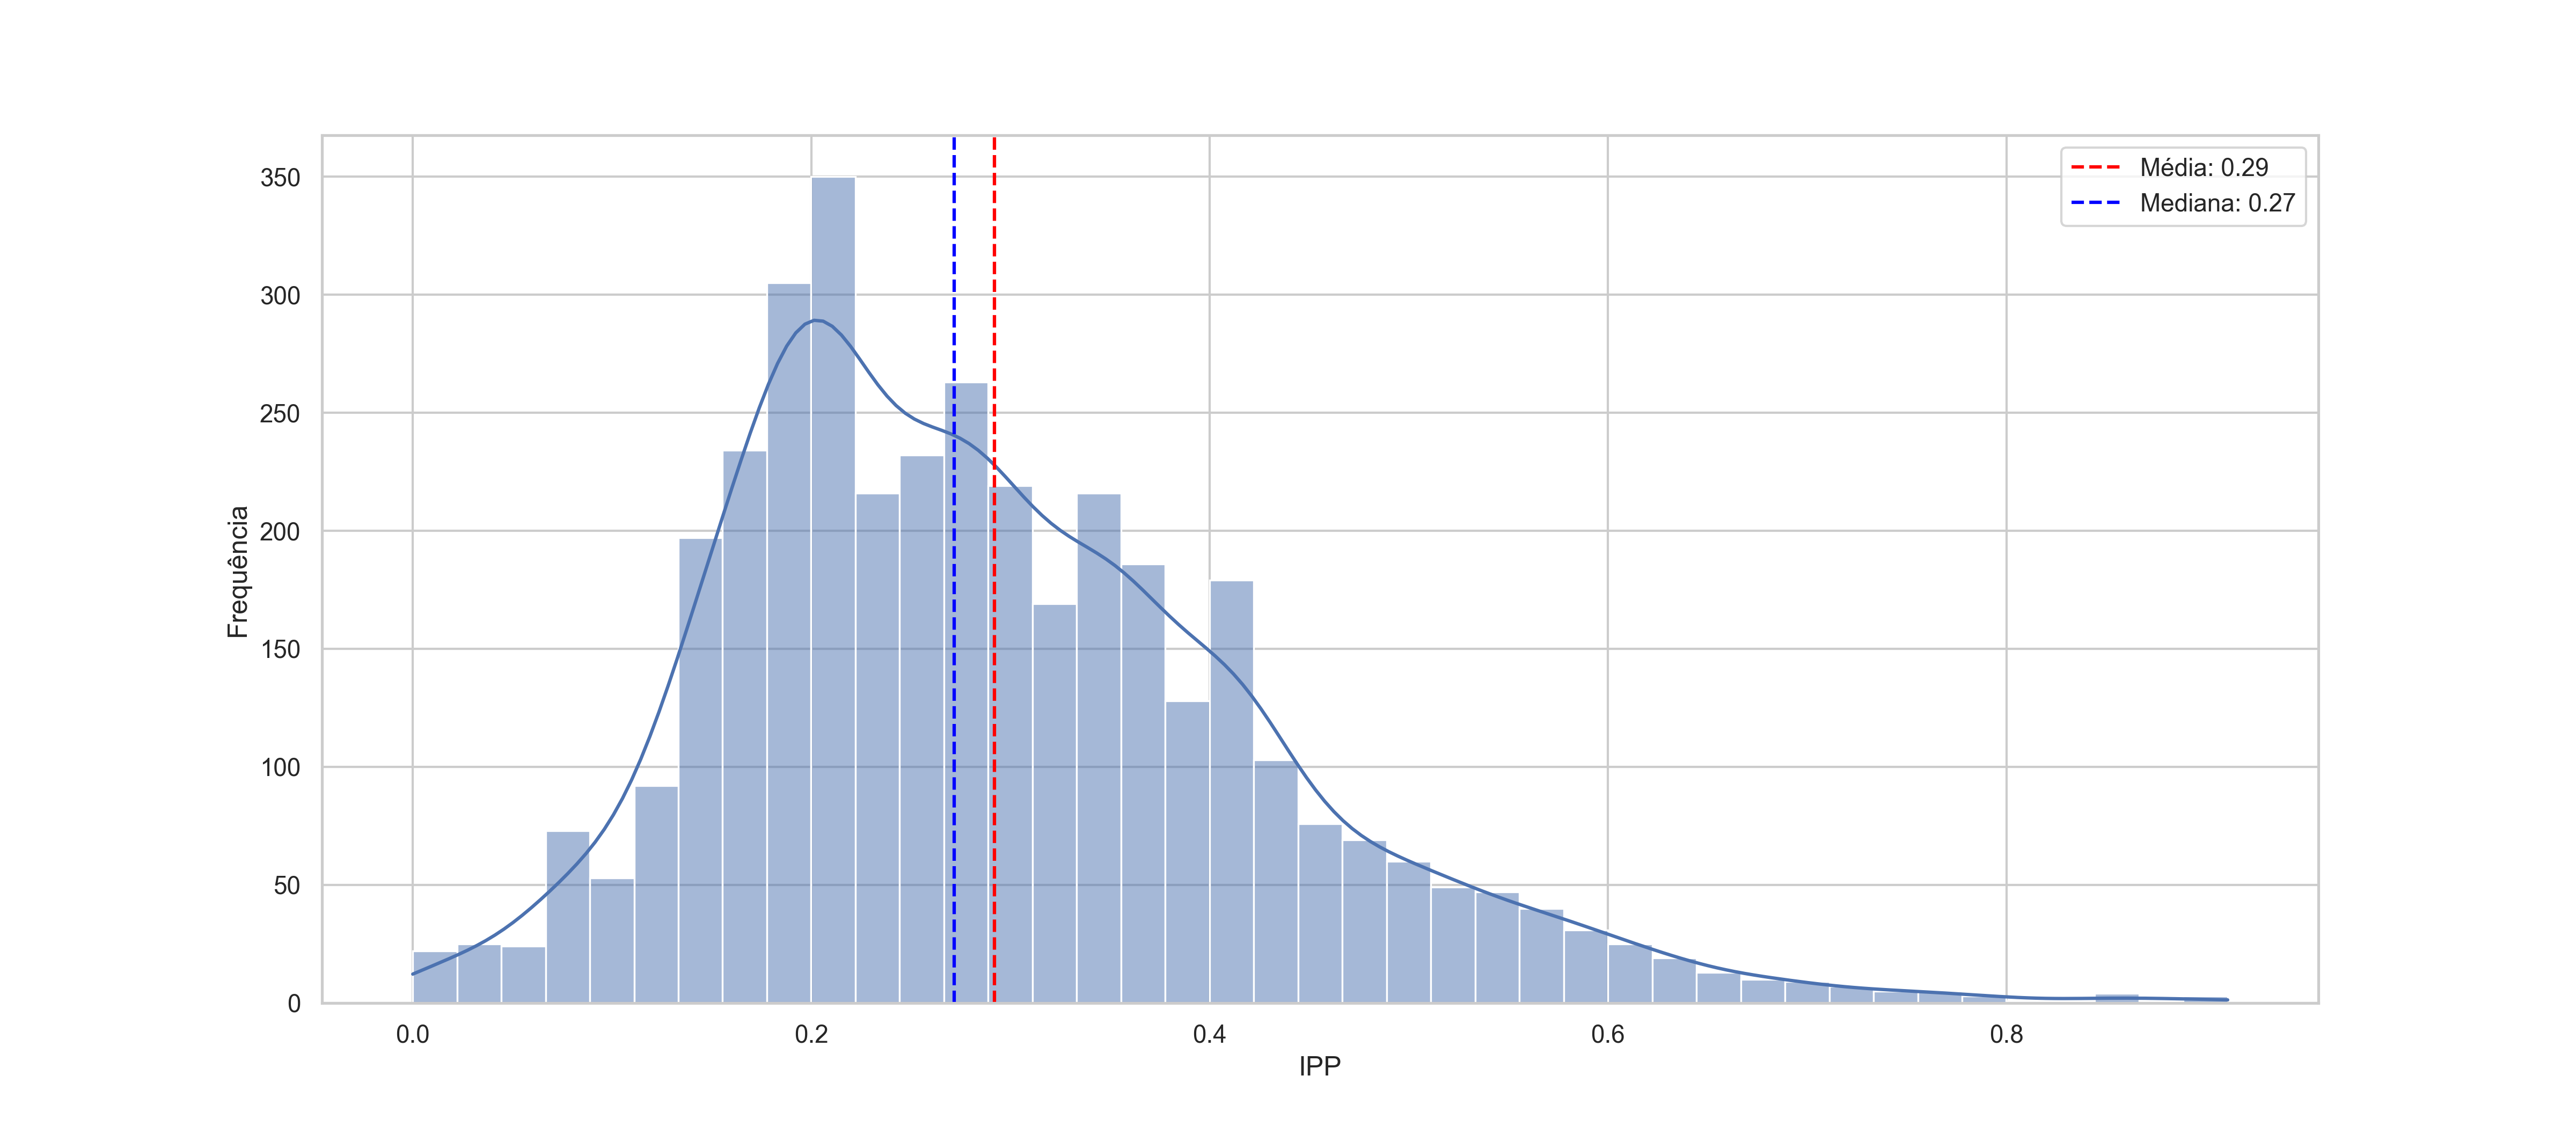
\includegraphics[width=0.95\linewidth]{figures/ipp_histplot.png}
    \end{center}
    \vspace{-0.5em}
  \end{frame}

  \begin{frame}{IPP — distribuição por legislatura}
    \begin{center}
      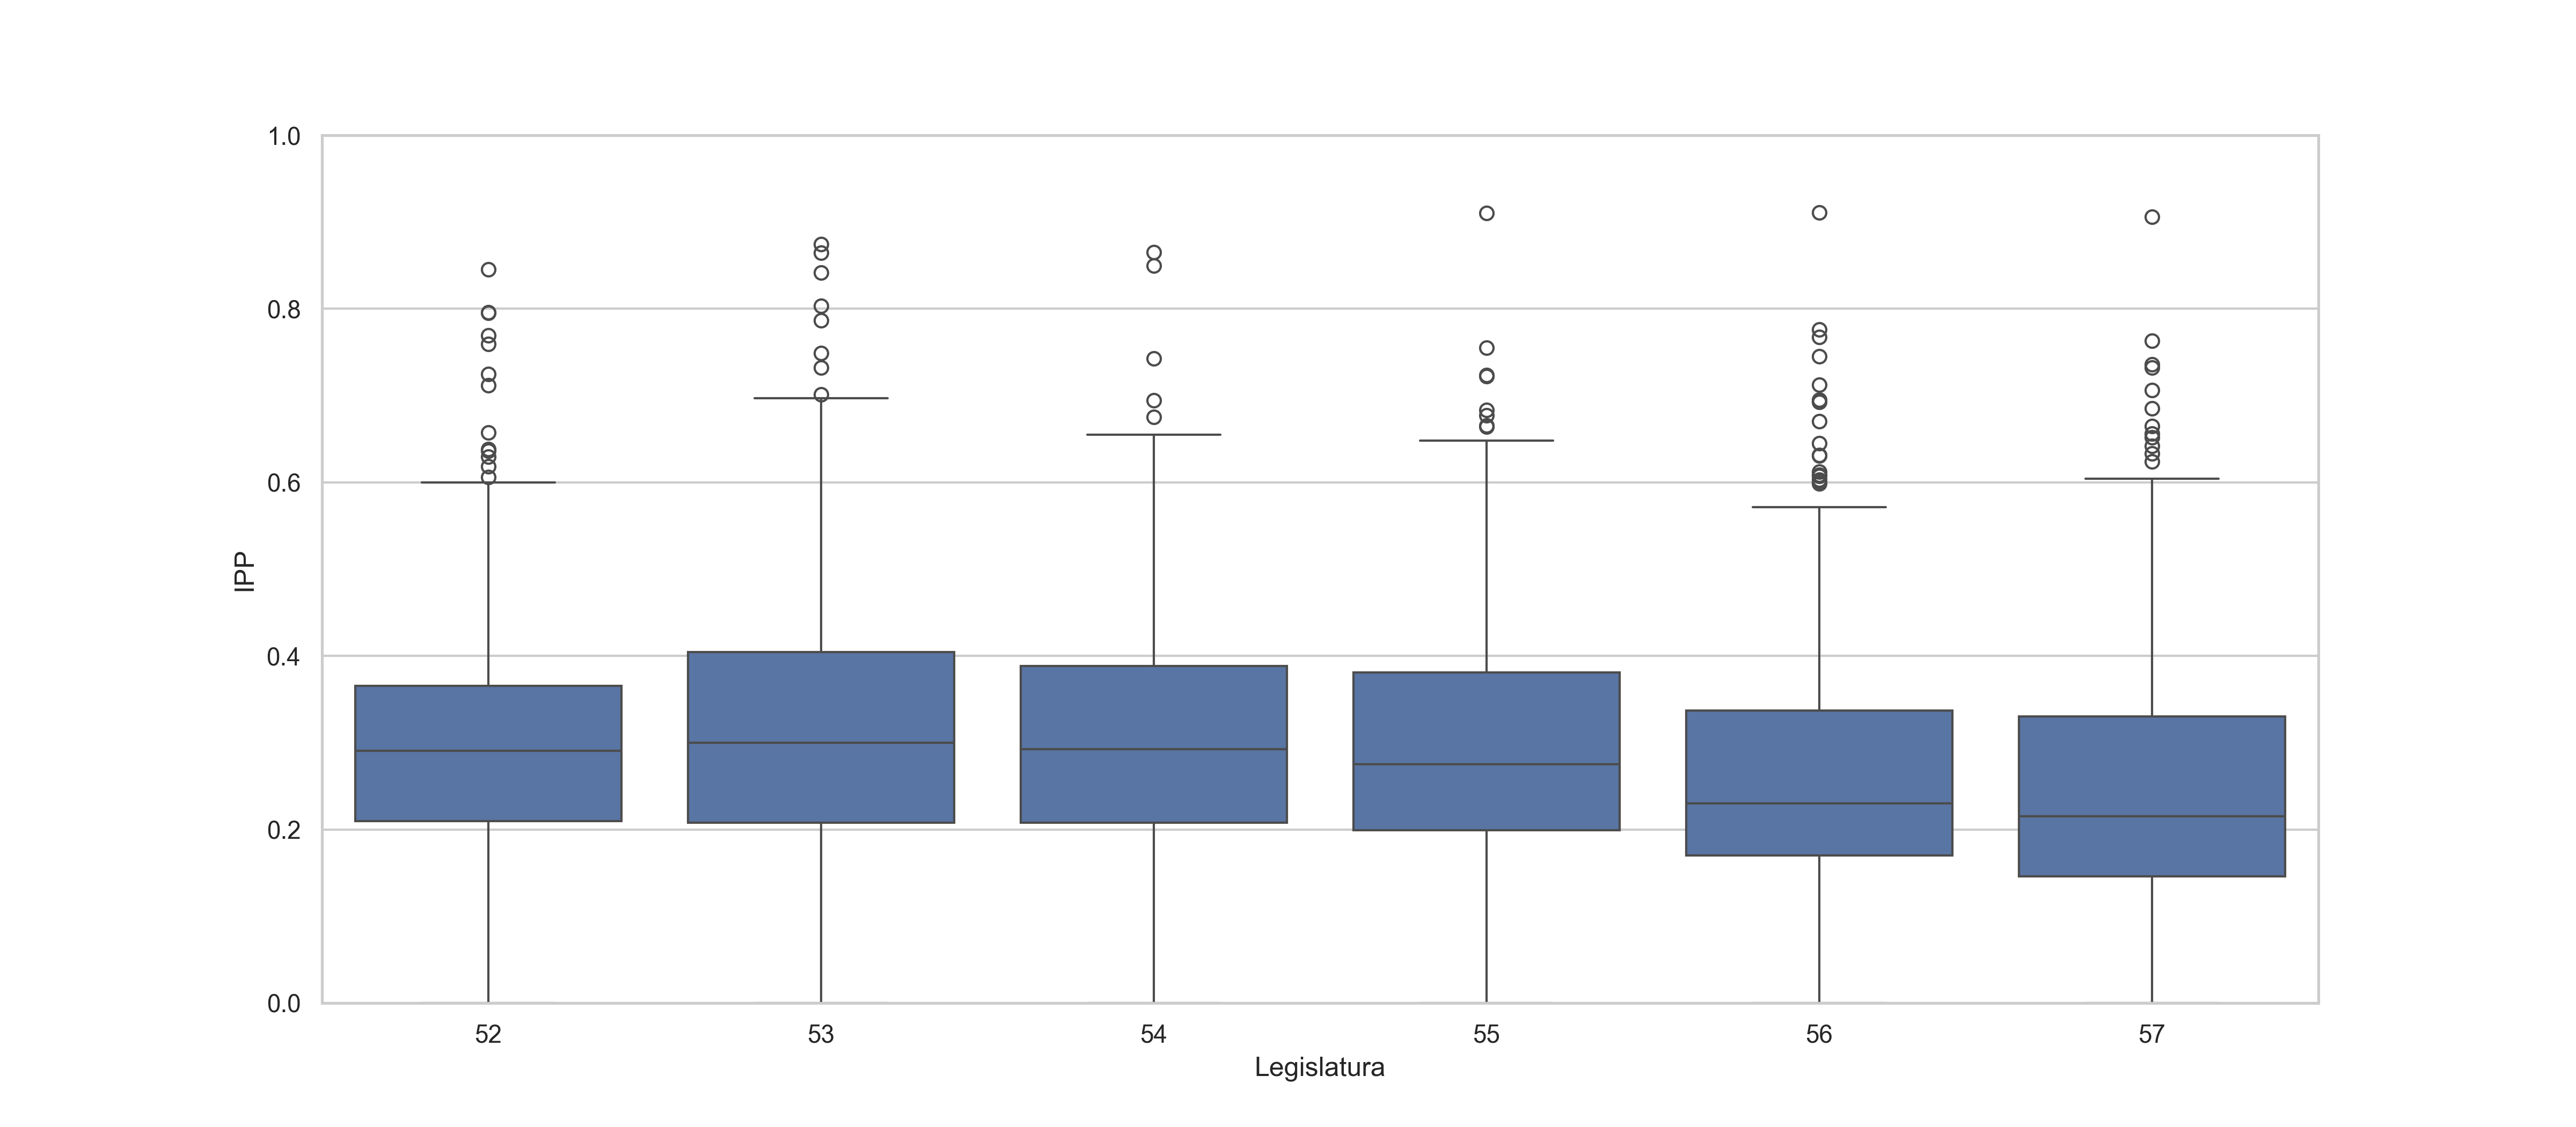
\includegraphics[width=0.95\linewidth]{figures/ipp_boxplot.png}
    \end{center}
    \vspace{-0.5em}
  \end{frame}

% ----------------------------------------------------------------------------
\section{IFS}

  \begin{frame}{IFS (em testes) — ideia geral}
    \begin{itemize}
      \item Construir uma base vetorial de conteúdos verificados como falsos (corpus rotulado por agências de checagem).
      \item Filtrar/curar o corpus para garantir qualidade (deduplicação, linguagem, contexto, datas, claims centrais).
      \item Comparar postagens de cada parlamentar com essa base vetorial via similaridade do cosseno (ou métrica afim) sobre embeddings.
      \item Definir um limiar $\tau$ de similaridade: acima de $\tau$ a postagem é potencialmente relacionada ao conteúdo falso ($\max_j \cos(e(\text{post}), e(\text{claim}_j))\geq\tau$).
      \item Classificar se a postagem \textit{propaga} ou \textit{denuncia} (classificador de \textit{stance}).
    \end{itemize}
  \end{frame}

  \begin{frame}{Definição operacional (versão inicial)}
    Para o parlamentar $i$, considere o conjunto de similaridades das postagens que superam o limiar e foram classificadas como \textit{propagação}:
    \[
      \mathcal{S}_i \,=\, \Big\{ s_{it} \;:\; s_{it} = \max_j \cos\big(e(\text{post}_{it}), e(\text{claim}_j)\big)\geq \tau,\; \text{stance}_{it}=\text{propaga} \Big\}.
    \]
    Também defina o total de postagens analisadas $P_i$ e a contagem de matches $c_i = |\mathcal{S}_i|$.
  \end{frame}

  \begin{frame}{Formas de pontuação (em avaliação)}
    \textbf{A) Incidência (contagem/taxa)}\\
    Pontua por ocorrência; retorna mais alto quanto menor a incidência.
    \[
      r_i \,=\, \frac{c_i}{P_i}\quad\Rightarrow\quad \mathrm{IFS}_i^{\text{taxa}} \,=\, 1 - r_i \;\in [0,1] \quad (\text{equiv.: } 1 - \tfrac{100\,c_i}{P_i\cdot 100}).
    \]
    \vspace{0.2em}
    \textbf{B) Distância (similaridade média)}\\
    Penaliza mais matches mais próximos dos claims falsos.
    \[
      \bar s_i \,=\, \begin{cases}
        \tfrac{1}{c_i}\sum\limits_{s\in\mathcal{S}_i} s, & c_i>0,\\
        0, & c_i=0
      \end{cases}
      \quad\Rightarrow\quad \mathrm{IFS}_i^{\text{dist}} \,=\, 1 - \bar s_i \;\in [0,1].
    \]
    \small Observações: pode-se usar top-$k$, ponderar por engajamento/recência e calibrar $\tau$. Ambas as variantes têm orientação \textit{quanto maior, melhor}.
  \end{frame}

  % \begin{frame}{Medidas auxiliares e variações}
  %   \begin{itemize}
  %     \item \textbf{Contagem}: $c_i = |\mathcal{S}_i|$ (número de matches de propagação), com taxa por 100 postagens.
  %     \item \textbf{Top-$k$}: usar $\bar s_i$ apenas dos $k$ maiores $s$ para robustez a ruído.
  %     \item \textbf{Peso por engajamento/recência}: média ponderada por curtidas, compartilhamentos e decaimento temporal.
  %     \item \textbf{Normalização de atividade}: controles por volume de postagens para comparabilidade entre parlamentares.
  %   \end{itemize}
  % \end{frame}

  \begin{frame}{Desafios e calibração}
    \begin{itemize}
      \item \textbf{Polaridade}: distinguir \textit{denúncia} de \textit{propagação}; requer rotulagem e/ou \textit{stance detection} supervisionada.
      \item \textbf{Limiar $\tau$}: calibrar via validação (ROC/PR), \textit{human-in-the-loop} e \textit{error analysis} (falsos positivos/negativos).
      \item \textbf{Cobertura do corpus}: garantir representatividade temporal e temática; atualização contínua.
      % \item \textbf{Transparência}: registrar exemplos de matches e explicações para auditoria pública.
    \end{itemize}
  \end{frame}




% ----------------------------------------------------------------------------
\section{Conclusão}
\begin{frame}{Conclusão}
  \begin{itemize}
    \item \textbf{IRD}: métrica transparente de \textit{representação descritiva} baseada em alvo populacional e pesos individuais; normalizável e comparável ao longo do tempo e entre legislaturas.
    \item \textbf{IPP}: síntese de \textit{especialização legislativa} e \textit{carreira} com normalização e pesos explícitos; evidência empírica via análise fatorial sustenta a estrutura bidimensional.
    \item \textbf{IFS (em testes)}: arquitetura para medir \textit{distância/incidência} de postagens em relação a notícias falsas, com limiar, classificação de polaridade e duas variantes de escore em $[0,1]$ (taxa e distância).
    \item \textbf{Uso integrado}: monitoramento por indivíduo/partido/bancada/legislatura; comparações temporais; identificação de padrões e outliers; insumos para comunicação e governança.
    \item \textbf{Cuidados e próximos passos}: curadoria do corpus (IFS), calibração de $\tau$ e \textit{stance}, testes de robustez de pesos (IPP), extensões multicategoria (IRD) e padronização de pipelines e painéis públicos.
  \end{itemize}
\end{frame}


% % ----------------------------------------------------------------------------
% \section{Apêndice}

% \begin{frame}{Reprodutibilidade}
%   \begin{itemize}
%     \item Cadernos: \texttt{studies/equality\_index/indice\_igualdade.ipynb}, \texttt{studies/ipp/ipp\_v2.ipynb}, \texttt{studies/ipp/analise\_fatorial\_v2.ipynb}.
%     \item Código: \texttt{src/indices/equality\_index\_calculator.py}, \texttt{src/indices/ipp\_calculator.py}.
%     \item Saídas: \texttt{outputs/}, figuras: \texttt{imagens/}.
%   \end{itemize}
% \end{frame}


% \begin{frame}{Próximos Passos}
%   \begin{itemize}
%     \item Expandir o Equality Index para múltiplas dimensões (gênero $\times$ raça).
%     \item Testes de robustez do IPP (pesos alternativos; AFC/IRT).
%     \item Integração com votações, redes e análises de coautoria.
%   \end{itemize}
% \end{frame}


\end{document}